% This is samplepaper.tex, a sample chapter demonstrating the
% LLNCS macro package for Springer Computer Science proceedings;
% Version 2.20 of 2017/10/04
%
\documentclass[runningheads]{llncs}
%
\usepackage{graphicx}
\usepackage{hyperref}

\begin{document}
%
\title{WASP - Windows and Shutters Project}

\author{Group 7: Sebastian Künzel \and
Lukas Nabakowski \and
Jannis Rapp}

\institute{Service Computing Department, IAAS, University of Stuttgart
\email{st150016@stud.uni-stuttgart.de} \and
\email{st148841@stud.uni-stuttgart.de} \and
\email{st150565@stud.uni-stuttgart.de}}
%
\maketitle              % typeset the header of the contribution
%
\begin{abstract}
The abstract should briefly summarize the contents of the report in
150--250 words. 

\keywords{First keyword  \and Second keyword \and Another keyword.}
\end{abstract}
%
%
%
\section{System Introduction}

Quality of Life and well-being is an essential factor for work performance and employees in modern office environments~\cite{employee_wellbeingimportant}. One prominent problem regarding indoor office buildings is a high CO$_2$ concentration which can lead to impaired work performance and negative health symptoms~\cite{indoor_polutionCO2}. Further possible disturbances in office environments include ambient noise and sunlight~\cite{indoor_noiselight}. Both elements distract the concentration of office workers. 
\newline
We use an intelligent windows and blinds management system to address the problems outlined above.
This system uses sensors to monitor the CO$_2$ concentration, ambient noise level, and sunlight intensity.
Based on the observed information, the system can then react by adjusting the windows, shutters, and heating accordingly.
\newline
The goal is to control the office's windows and shutters to maintain high air quality with a low CO$_2$ concentration and a comfortable temperature while avoiding distractions caused by ambient noise and blinding sunlight. The system is also equipped to adapt to environmental influences (e.g. rain and wind) that can adversely affect the indoor office space when windows are open.   



\section{System Analysis}

\begin{description}
\item{\textbf{Must have requirements}}\
\begin{itemize}
    \item [R1.] Maintaining low CO$_2$ concentrations
    \item [R2.] User has manual control of windows, blinds, and heating
    \item [R3.] User can specify automation parameters
    \item [R4.] Sustaining desired room temperature using energy efficient decisions
    \item [R5.] Great amounts of sunlight are blocked by blinds
    \item [R6.] Prevent rain through open windows
\end{itemize}
\item{\textbf{Nice to have requirements}}\
\begin{itemize}
    \item [R7.] System status overview 
    \item [R8.] Prevent strong wind from coming through windows 
    \item [R9.] Prevent distracting amounts of ambient noise
    \item [R10.] Plan ahead by using a weather forecast 
\end{itemize}
\end{description}
\subsection{Must have requirements}
\subsubsection{R1. Maintaining a low CO$_2$ concentration}

Ensuring the well-being of employees by avoiding high levels of CO$_2$ is one of the essential problems the window management system is supposed to address. Therefore, it is a core requirement that the system is able to maintain low CO$_2$ levels inside the office space.

\subsubsection{User has manual control of windows, blinds, and heating}
\begin{itemize}
    \item [U1:] \label{r2u1} \textit{As a project lead, I need a dark room so that my Power Point presentations are clearly visible.}
    \item [U2:] \label{r2u2} \textit{As a safety manager, I need to open the windows in case of an emergency.}
\end{itemize}
While the system aims at automating all window, blinds, and heating functionality optimally, there do exist scenarios, where the manual operation of these devices is desired. Detection and response to all scenarios is not possible due to the limited scope of the system. The user stories~\hyperref[r2u1]{U1} and~\hyperref[r2u1]{U2} detail such scenarios where manual control is needed. 

\subsubsection{User can specify automation parameters}
Different office environments have different demands regarding acceptable CO$_2$, ambient noise levels, etc. These demands can only be satisfied, by adjusting the automation accordingly.

\subsubsection{Sustaining desired room temperature using efficient decisions}
\begin{itemize}
    \item [U1:] \label{r4u1} \textit{As a CEO, I want the system to operate energy efficient, so that I can minimize my heating costs.}
\end{itemize}
Sustaining a desired temperature contributes to the well-being of employees in the office space. Additionally user story~\hyperref[r4u1]{U1} demonstrates the need to take energy efficiency into account during the systems operation.
Therefore coordination between windows and heating is necessary.

\subsubsection{Great amounts of sunlight are blocked by blinds}
\begin{itemize}
    \item [U1:] \label{r5u1} \textit{As an employee, I want shades to be in a position so that i am not blinded by sunlight.}
\end{itemize}
Blinding sunlight can be a distraction to workers in the office space~\cite{indoor_noiselight} the argument to block excessive amounts of sunlight is further reinforced by user story~\hyperref[r5u1]{U1}. The effect of sunlight can prevented by the use of blinds. Considering the fact, that blinds are a part of the systems automation objective it is therefore necessary, that the system automatically blocks excessive sunlight.

\subsubsection{Prevent rain through open windows}
Open windows inherently create the risk of rain coming into the office and damaging the interior. In order to prevent damage to the office interior the system has to detect rain and prevent it from entering the building.

\subsection{Nice to have requirements}
\subsubsection{System status overview}
\begin{itemize}
    \item [U1:] \label{r6u1} \textit{As a facility manager, I want to be able to view the status of different system components, so that I don't have to control them manually.}
    \item [U2:] \label{r6u2} \textit{As a security officer, I want to be able to the view current state of the windows, so that I can make sure that nobody can get in.}
\end{itemize}
Both the security officer~\hyperref[r6u1]{(U1)} and the facility manager~\hyperref[r6u1]{(U2)} have an interest in a system overview functionality, as it would make their respective work easier. But they are both also able to perform their job without this functionality. It is therefore nice to fulfill this requirement but not requisite to the systems functionality.

\subsubsection{Prevent strong wind from coming through windows}
While strong wind can be nuisance it has no negative effect on the office workers health and is easier to notice than CO$_2$. It would therefore be nice to avoid strong wind but is not necessary for the success of the system. 

\subsubsection{Prevent distracting amounts of ambient noise}
Ambient noise can be very distracting closing the windows during peak ambient noise levels can reduce outside noise significantly. Ambient noise depends on the office location and is generally less essential to the system's operation.

\subsubsection{Plan ahead by using a weather forecast}
Being able to plan around bad weather situations would enhance the systems ability to satisfy set goals. At time this requirement is not needed for the systems base functionality. It is therefore not mandatory.   


\newpage


\begin{itemize}
    \item [U1:] \textit{As a project lead, I need a dark room so that my Power Point presentations are clearly visible.}
    \item [U2:]\label{test} \textit{As a project lead, I need a dark room so that my Power Point presentations are clearly visible.}
\end{itemize}

\section{System Architecture Design}












The performance and health of office employees can be increased my monitoring the CO2 concentration, aswell   

To increase the performance and health of employees an automated  



Modern companies are focus




Describe the scope (ghdfghfdhgbackground information and problem statement) and the goals of your project.

Table~\ref{tab1} an example of a table.

\begin{table}
\caption{Table captions should be placed above the
tables.}\label{tab1}
\begin{tabular}{|l|l|}
\hline
Item & Deadline \\
\hline
I111 & D1 \\
I2 & D2 \\
I3 & D3 \\
I4 & D4 \\
I5 & D5 \\
\hline
\end{tabular}
\end{table}

Fig.~\ref{fig1} gives an example of a figure.

\begin{figure}
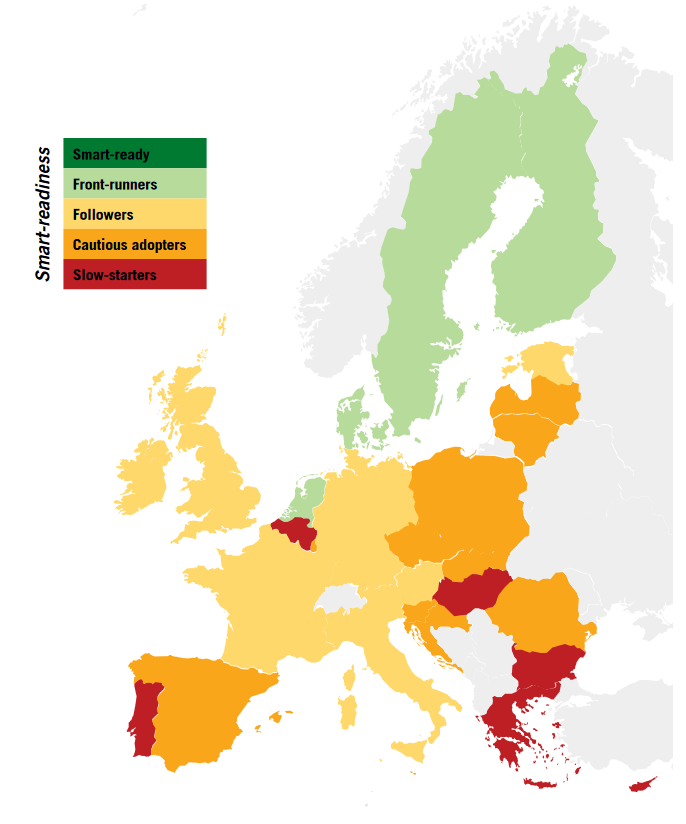
\includegraphics[width=\textwidth]{fig1}
\caption{A figure caption is always placed below the illustration.
Please note that short captions are centered, while long ones are
justified by the macro package automatically.} \label{fig1}
\end{figure}

For citations of references, we prefer the use of square brackets
and consecutive numbers. The following bibliography provides
a sample reference list with entries for journal
articles~\cite{ref_article1}, a book~\cite{ref_book1}, proceedings without editors~\cite{ref_proc1},
and a homepage~\cite{ref_url1}. Multiple citations are grouped
\cite{ref_article1,ref_book1},
\cite{ref_article1,ref_book1,ref_proc1,ref_url1}.

\section{System Analysis}
Describe the user requirements of your system.

\section{System Architecture Design}
Describe and provide a design of the architecture of your system.

\section{System Implementation}
Describe the implementation of your system. This section is only relevant for the report and should be omitted for the project description. 

\section{Discussion and Conclusions}
Here you can discuss some interesting points or limitations of your system and conclude the report.

%
% ---- Bibliography ----
%
\bibliographystyle{splncs04}
\bibliography{mybib}

All links were last followed on April 17, 2020.

\end{document}
